\documentclass[../document.tex]{subfiles}
 
\begin{document}
\subsection{Schwingungen}

Als Schwingung bezeichnet man eine Hin- und Herbewegung um eine Ruhelage.
Statt Schwingung kann auch Oszillieren verwendet werden.
Das sich Bewegende Stück wird als Oszillator bezeichnet und benötigt folgende Eigenschaften um zu Schwingen:
\begin{itemize}
	\item auslenkende Kraft (Krafteinwirkung von Außen, z.B.: Pendel anheben)
	\item rückstellende Kraft (z.B.: Feder- oder Schwerkraft)
	\item Trägheit
\end{itemize}

\subsubsection{Gedämpfte Schwingung}
Durch Energieverlust (Reibung) hört der Oszillator langsam wieder auf zu oszillieren. Dadurch ergibt sich eine ungedämpfte Schwingung

$y = r e^{-\delta t} \sin(\omega t + \phi)$
\begin{itemize}
	\item $y$: momentange Auslenkung
	\item $r$: Amplitude
	\item $\delta$: Dämpfungskonstante
	\item $\omega = 2\pi f = \frac{2\pi}{T}$: Kreisfrequenz
	\item $\phi$: Phasenwinkel
\end{itemize}

\subsubsection{Ungedämpfte Schwingung}
Um eine ungedämpfte Schwingung zu erhalten muss dem Oszillator regelmäßig im richtigen Moment die durch Reibung verloren gegangene Energie zugeführt werden.
Je nachdem ob der Körper selber die Energie aufbringt oder nicht spricht man von einer selbst erregten Schwingung oder einer erzwungenen Schwingung.

Dabei gibt $T$ die Schwingungsdauer in Sekunden an und errechnet sich wie folgt:
$T = \frac{1}{f}$

\subsubsection{Energieform bei Schwingungen}
Bei einem Pendel wird zwischen potentieller und kinetischer Energie umgewandelt. Dabei ist die potentielle Energie am kleinsten wenn das Pendel am tiefsten Punkt angelangt ist (Ruhelage). 
Umgekehrt ist die kinetische Energie am kleinsten wenn das Pendel seine maximale Auslenkung erreicht hat. 

$E_{pot} = \frac{D y^2}{2}$\\
$E_{kin} = \frac{m v^2}{2}$\\
$E_{gesamt} = E_{pot} + E_{kin} + U = const$\\

\begin{itemize}
	\item $D = k$: Richtgröße
	\item $y$: momentane Auslenkung
	\item $m$: Masse
	\item $v$: Geschwindigkeit
	\item $U$: innere Energie
\end{itemize}

\subsubsection{Energieformen bei speziellen Schwingungen}

\textbf{Fadenpendel}

Wie man an der Formel sehen kann ist die Schwingfrequenz eines Fadenpendel nicht abhängig von seiner Masse. Die Frequenz nimmt ab je länger der Faden ist.

$ f_0 = \frac{1}{2\pi} \sqrt{\frac{g}{l}}$\\
$ F = 2\pi\sqrt{\frac{l}{g}}$

\begin{itemize}
	\item $l$: Länge des Fadens
	\item $g$: Erdbeschleunigung $9.81 m/s $
\end{itemize}

\textbf{Federpendel}

$ f = \frac{1}{2\pi} \sqrt{\frac{k}{m}}$\\
$ F = 2\pi\sqrt{\frac{m}{k}}$

\begin{itemize}
	\item $k$: Federkonstante
	\item $m$: Masse
\end{itemize}

\subsubsection{Erzwungene Schwingung}

Bei einer erzwungenen Schwingung muss das Pendel einer Erregerfrequenz $f_E$ folgen.

\begin{itemize}
	\item Wenn $f_E < f_0$ dann folgt das Pendel dem Erreger genau
	\item Wenn $f_E = f_0$ Resonanzfall -> Resonanzkatastrophe
	\item Wenn $f_E > f_0$ sehr kleine Amplitude, der Erreger ist zu schnell
\end{itemize}

\subsubsection{Resonanzerscheinungen}
\textbf{Erwünscht bei:} Funkempfang, Ultraschall, Mikrophon?

\textbf{Unerwünscht bei:} Verkehrslärm, Maschieren im Takt - Brücken können einstürzen, Dröhnen von Teilen eines Fahrzeug - Lockerung, "hämmerndes Geräusch" wenn Autofenster bei hoher Geschwindigkeit geöffnet ist.

Eine Resonanzkatastrophe tritt auf wenn die Amplitude eines durch eine periodische Kraft zu Schwingungen gezwungener Oszillator so groß wird, dass er sich selbst zerstört.

Wenn zwei Pendel über eine Feder gekoppelt werden und eines der Pendel ausgelenkt wird finden eine Amplitudenübertragung auf das zweite Pendel statt wodurch das ursprünglich ausgelenkte Pendel aufhört zu schwingen und das andere anfängt. Dieser Vorgang wiederholt sich dann wieder in die andere Richtung.

\subsection{Wellen}
Eine Welle ist eine zeitliche und räumliche Veränderung eines Schwingungszustandes. Die Ausbreitungsgeschwindigkeit wird mit $c$ bezeichnet. Eine Welle transportiert Energie.
\subsubsection{Mechanische Wellen}
Ist eine Folge von Schwingungen die sich in einem Medium ausbreitet. Ein Medium ist ein fester/flüssiger oder gasförmiger Stoff.

\begin{itemize}
	\item \textbf{Transversalwellen} (Querwellen)\\
	z.B.: Wasserwellen, Erdbeebenwellen
	\item \textbf{Longitudinalwellen} (Längswellen)\\
	z.B.: Schallwellen, Dichtewellen, Druckwellen, Erdbeebenwellen
\end{itemize}

Die Beschreibungsgrößen von Wellen sind:
\begin{itemize}
	\item $\lambda$: Wellenlänge in m
	\item $c$: Die Ausbreitungsgeschwindigkeit in m/s
	\item $f$: Die Frequenz in Hertz (Anzahl der Schwingungen pro Sekunde)
	\item $T$: Die Schwingungsdauer in s (Zeitdauer einer vollständigen Hin-/Zurückbewegung)
	\item $r$: Die Amplitude in m (max. Auslenkung/Abstand zur Ruhelage)
\end{itemize}

Bei einer Stoßwelle breitet sich die Welle nach einer einmaligen Störung aus
Eine periodischen Welle wird bei einer periodischen Erregung erzeugt.

\textbf{Beschreibung von Wellen}
\begin{itemize}
	\item \textbf{Wellenzentrum} Ist der Ort des Erregers, von dem sich die Welle ausbreitet\\z.B.: Lichtquelle, Stein ins Wasser
	\item \textbf{Wellenfront} Verbindet alle Punkte der Welle mit gleicher Phasenlage
	\item \textbf{Wellenvektoren} Stehen senkrecht auf der Wellenfront und geben die Ausbreitungsrichtung der Welle an.
\end{itemize}

\textbf{Ausbreitungsgeschwindigkeit einer Stoßwelle}
\begin{itemize}
	\item Je größer die mechanische Spannung als Maß für die Kopplung, umso schneller breitet sich die Stoßwelle aus.
	\item Je größer die Dichte, umso niedriger ist die Ausbreitungsgeschwindigkeit.
\end{itemize}

Die Ausbreitungsgeschwindigkeit von Wellen $c = \sqrt{\frac{Kopplungsmaß}{Traegheitsmass}}$

\subsubsection{Das Prinzip von Huygens}

Eine Welle breitet sich aus, indem von jedem ihrer Punkte eine neue allgemeine (halb)kugelförmige Elementarwelle ausgeht. Durch Interferenz aller Elementarwellen ergibt sich die tatsächlich beobachtete Welle. Dadurch wird Beugung und Brechung erklärt.

\subsubsection{Überlagerung von Schwingungen/Wellen}
auch Interferenz gennant. Es gibt:
\begin{itemize}
	\item \textbf{konstruktive Interferenz}: gleichzeitige Wellenberg/Täler - die Welle verstärkt sich.
	\item \textbf{destruktive Interferenz}: verschobene Wellenberge/Täler - die Welle löscht sich aus.
\end{itemize}


\subsubsection{Stehende Welle}

Eine Stehende Welle ist eine Welle, deren Auslenkung an bestimmten Stellen immer Null beträgt. Diese Punkte werden auch Wellenknoten oder Schwingungsknoten genannt. Sie kann als Überlagerung zweier gegenläufig fortschreitender Wellen gleicher Frequenz und Amplitude verstanden werden. Die gegenläufigen Wellen können aus zwei verschiedenen Erregern oder durch Reflexion einer Welle an einem Hindernis entstehen. 

Bei einer Reflexion an einem festen Ende tritt ein Phasensprung von $\pi$ auf. Wenn also eine Welle zwischen zwei Fixpunkten reflektiert wird entsteht eine stehende Welle. Diese stehenden Wellen können aber nur ein vielfaches der Frequenz der Grundwelle haben. Anders gesagt, der Abstand zwischen A und B beträgt ein vielfaches der Wellenlänge. Damit ist gewährleistet das sowohl A als auch B Wellenknoten sind.

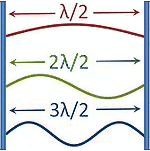
\includegraphics[width=4cm]{stehende_welle.png}












\end{document} 